%"###############################################
%
% Classification comparaison Qmax
%
%###############################################

\begin{figure}[h]
    \begin{minipage}[c]{.46\linewidth}
        \centering
        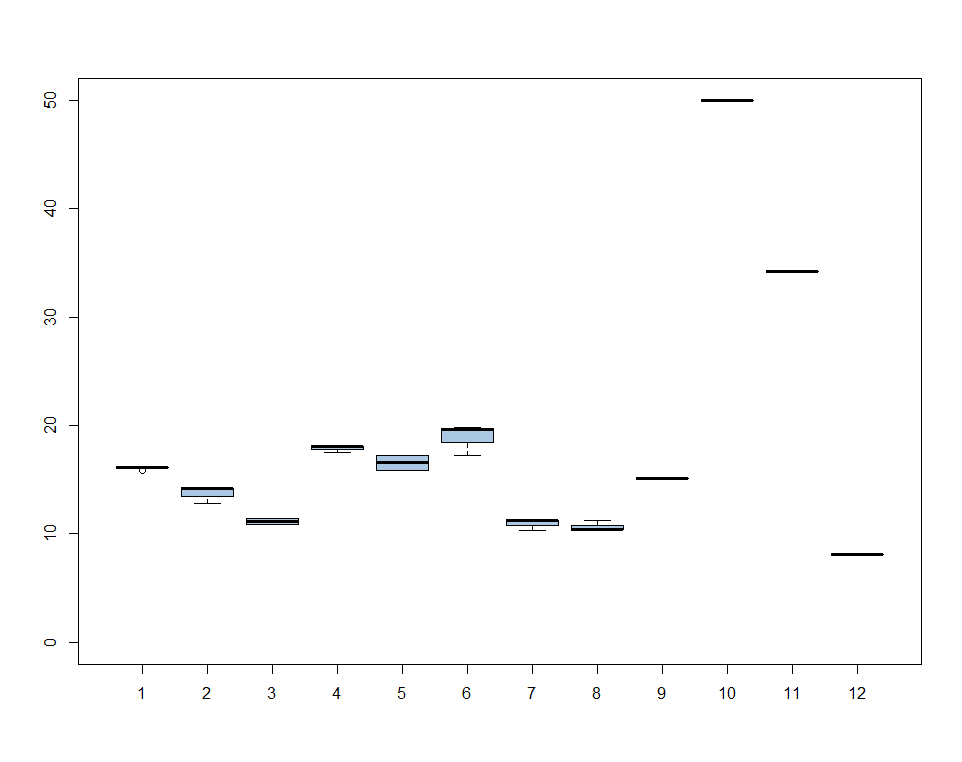
\includegraphics[width=1\textwidth]{../Fig/RTUPB/rtupb-qmax-k12-distribution.png}
        \caption{Distribution Qmax à 12 moins RTUPB}
    \end{minipage}
    \hfill%
    \begin{minipage}[c]{.46\linewidth}
        \centering
        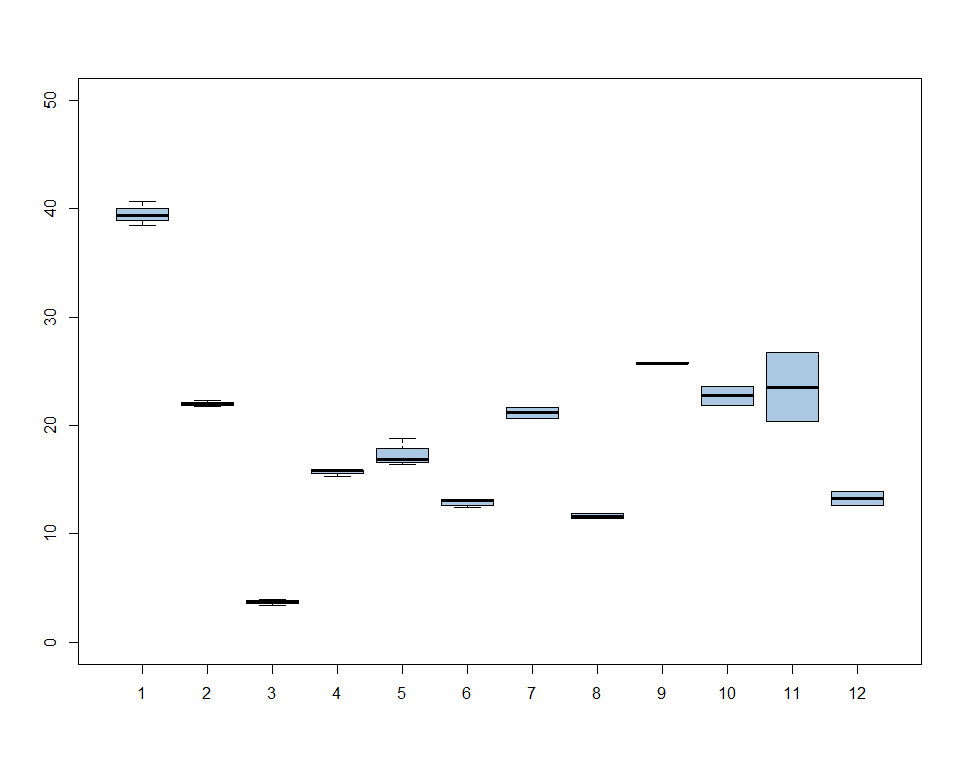
\includegraphics[width=1\textwidth]{../Fig/VPPBS/vppbs-qmax-k12-distribution.png}
        \caption{Distribution Qmax à 12 moins VPPBS}
    \end{minipage}
\end{figure}

%"###############################################
%
% Interpretation des trois figures RTUPB pre 
%
%#############################################




%\begin{figure}[h]
%    \begin{minipage}[c]{.46\linewidth}
%        \centering
%        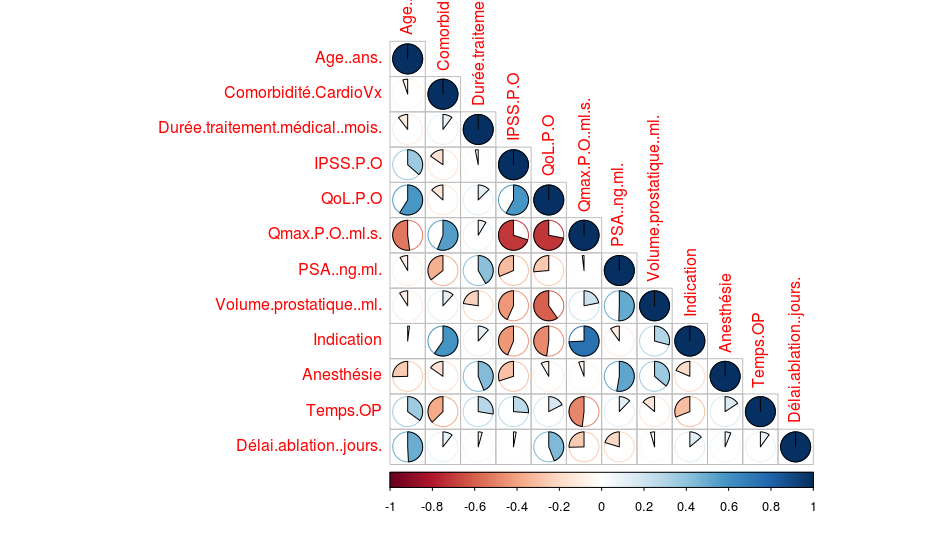
\includegraphics[width=1\textwidth]{../Fig/VPPBS/vppbs-corr-matrice-pie}
%        \caption{Légende}
%    \end{minipage}
%    \hfill%
%    \begin{minipage}[c]{.46\linewidth}
%        \centering
%        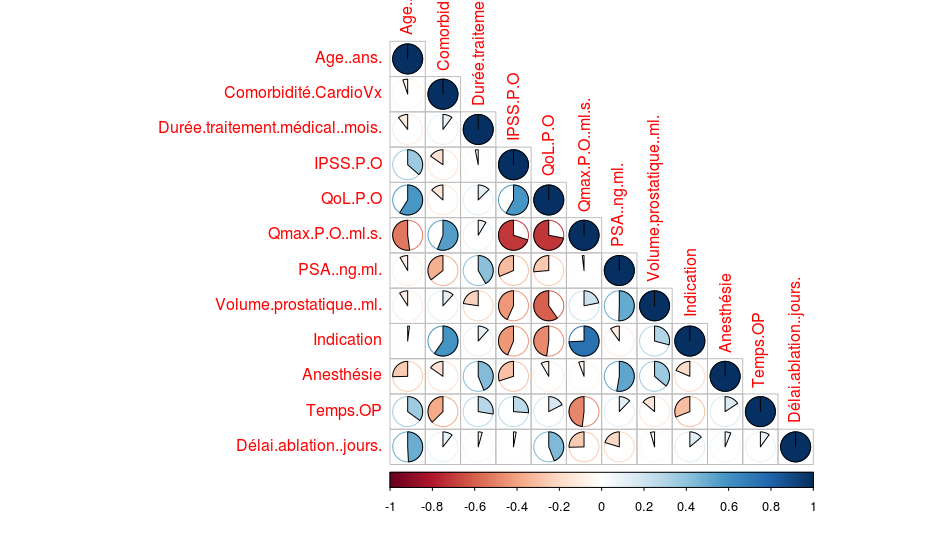
\includegraphics[width=1\textwidth]{../Fig/VPPBS/vppbs-corr-matrice-pie}
%        \caption{Légende}
%    \end{minipage}
%\end{figure}





%
%##########################
%# CONCLUSION
%##########################
